\documentclass[12pt]{article}
\usepackage[utf8]{inputenc}
\usepackage{graphicx}
\graphicspath{ {./resources/} }
\usepackage[a4paper,width=150mm,top=25mm,bottom=25mm]{geometry}
\usepackage{hyperref}
\hypersetup{
    colorlinks=true,
    linkcolor=blue,
    filecolor=magenta,      
    urlcolor=cyan,
    pdftitle={Overleaf Example},
    pdfpagemode=FullScreen,
}
\usepackage{listings}
\lstset{language=[Sharp]C,keywordstyle={\bfseries \color{blue}}}

\title{
{
\includegraphics[width=10cm]{logo.png}}

{Unity Developer Position Assessment}
}

\author{Mathias Wagner Nielsen & Simonas Holcmann}

\begin{document}

\maketitle

\section{Purpose of this document}
This is the specification for the Unity Developer Position Assessment.
The goal of this document is to faciliate a proper assessment of the applicant's ability to contribute to our Unity Development team.
This document is intended as a suggestion for how to demonstrate your fitness for the project to us.
If you want to demonstrate it in a better way, you're free to do so, but keep in mind that we have included these items for a reason.

\section{Rock, Paper, Scissors}
The task that we want you to complete is to write the code for a Rock, Paper, Scissors game.
We have provided a base repository that you must start from.
This base repository includes several packages:
\begin{itemize}
    \itemsep-0.5em
    \item Zenject
    \item UniRx
    \item UniTask
\end{itemize}

\paragraph*{}
\href{https://github.com/modesttree/Zenject}{Zenject} is a framework for dependency injection in Unity.
It is used extensively in our Unity software.
The main goal of using Zenject is to facilitate writing robust, testable code.
We have written a Zenject installer which binds the UI components in the scene to different classes that we call \verb|Presenters| (e.g. \verb|PlayerInputPresenter|).

\paragraph*{}
\href{https://github.com/neuecc/UniRx}{UniRx} is Reactive Extensions (Rx) ported to Unity.
One pattern that could be useful here is the \href{https://github.com/neuecc/UniRx#model-view-reactivepresenter-pattern}{MVRP pattern}.

\paragraph*{}
\href{https://github.com/Cysharp/UniTask}{UniTask} is a package providing better integration for async/await in Unity.
Asynchronous operations with a return value are best represented with a \verb|UniTask| (e.g. HTTP requests).

\begin{figure}[h!]
    \centering
    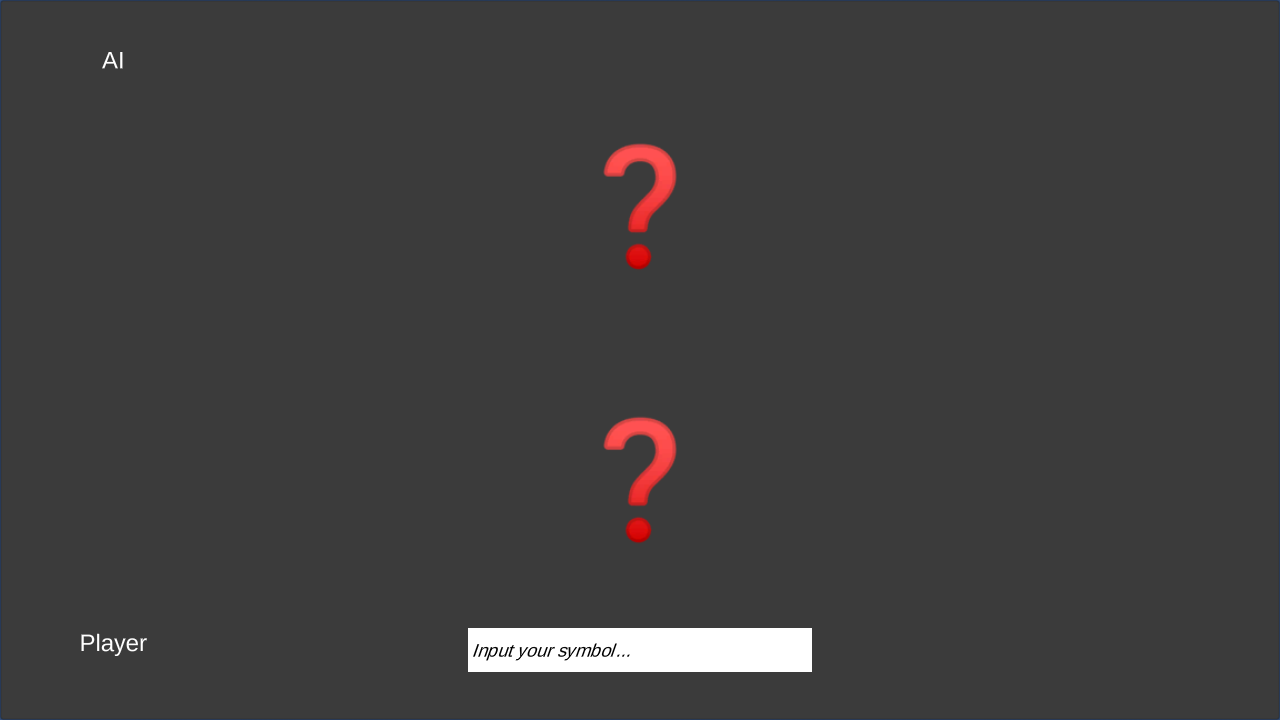
\includegraphics[width=0.7\textwidth]{input.png}
    \caption{The player must choose a valid symbol (rock, paper, or scissors)}
\end{figure}

\begin{figure}[h!]
    \centering
    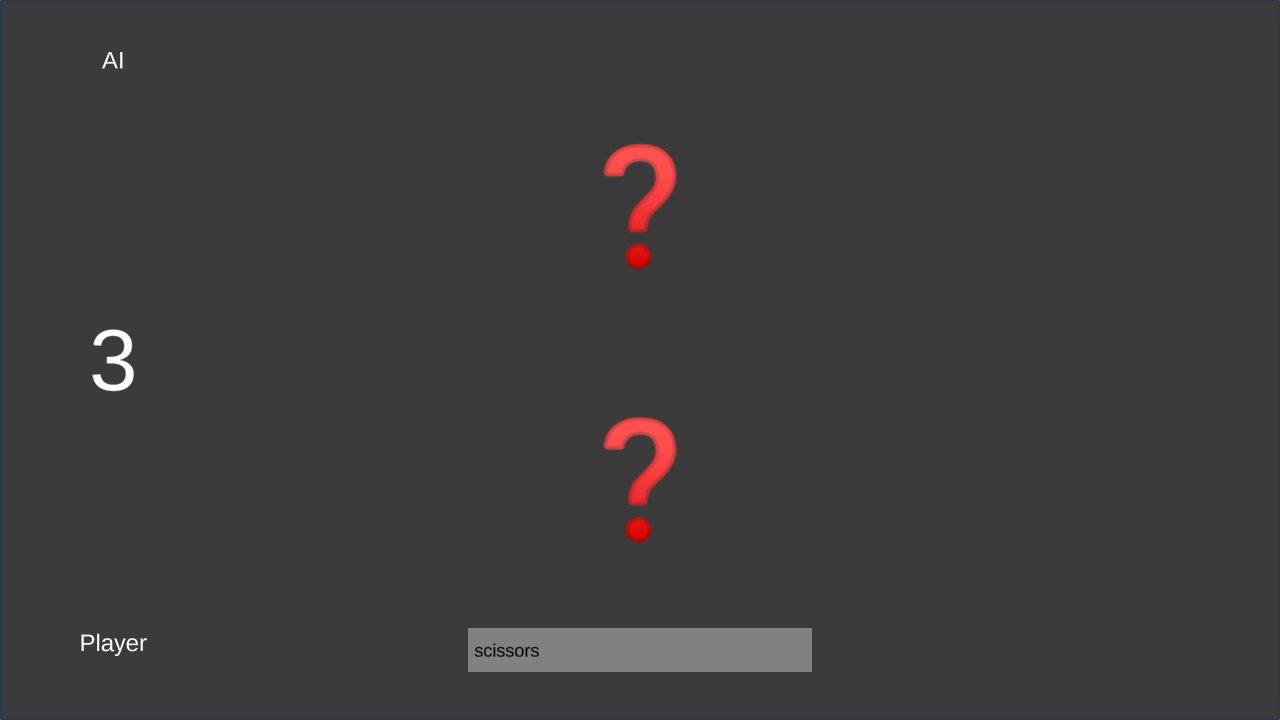
\includegraphics[width=0.7\textwidth]{countdown.png}
    \caption{A countdown is displayed while the AI chooses its move}
\end{figure}

\begin{figure}[h!]
    \centering
    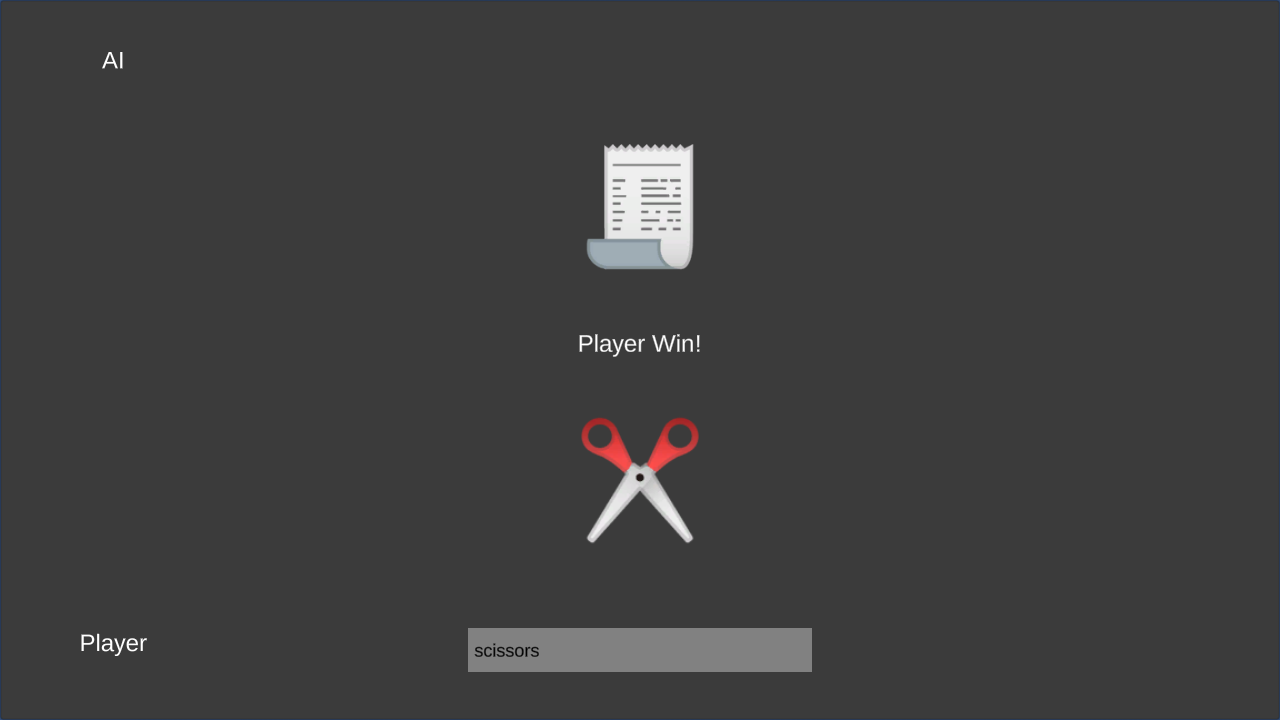
\includegraphics[width=0.7\textwidth]{player-win.png}
    \caption{The player wins}
\end{figure}

\clearpage
\paragraph*{The flow of the application:}
\begin{enumerate}
    \item The user inputs one of these values ['rock','paper','scissors'] into the input field.
    \item When the user presses 'Enter' on their keyboard, the answer is submitted, and the Player has locked in their chosen symbol. The program decides what symbol should be shown, based on the input. (However, does not show it yet).
    \item The AI sends an HTTP request to this website:
          \url{http://www.randomnumberapi.com/api/v1.0/random?min=0&max=2&count=1},
          and retrieves a random unsigned integer, from 0 (inclusive) to 2 (inclusive) ([0,1,2]).
    \item Based on the integer, the program chooses one of the three symbols. (However, does not show it yet).
    \item A countdown from 3 to 0 starts.
          When the timer hits 0, the question mark symbols turn into the respective rock, paper, scissors symbols for both players.
    \item After the symbols are shown, there is a 0.5 second delay, and the program announces who won the match. \par
          If the Player wins, the 'Result Text' should state 'Player Win!'. \par
          If the AI wins, the 'Result Text' should state 'AI Win!'. \par
          If it's a tie, the 'Result Text' should state 'Tie!'. \par
    \item The timer, input field value, and the rock paper scissors symbols get reset to their initial values (timer to being disabled, input field to empty, symbol image to question mark sprite).
\end{enumerate}

\paragraph*{We need to test the application. Write unit tests that prove that:}
\begin{enumerate}
    \item Input values ['rock','paper','scissors'] return the correct symbol.
    \item Matching two symbol values gives a correct output, for example, rock beats scissors, rock is equal to rock, paper beats scissors, etc.
    \item The HTTP request made to the \url{www.randomnumberapi.com} returns only values from 0 (inclusive) to 2 (inclusive).
\end{enumerate}

\section{Forking}
When writing your submission, please fork this project, clone your own fork, and commit your code to that. This way, you can share the forked repository with us.

\end{document}
